% Options for packages loaded elsewhere
\PassOptionsToPackage{unicode}{hyperref}
\PassOptionsToPackage{hyphens}{url}
%
\documentclass[
  ignorenonframetext,
  aspectratio=1610,
]{beamer}
\usepackage{pgfpages}
\setbeamertemplate{caption}[numbered]
\setbeamertemplate{caption label separator}{: }
\setbeamercolor{caption name}{fg=normal text.fg}
\beamertemplatenavigationsymbolsempty
% Prevent slide breaks in the middle of a paragraph
\widowpenalties 1 10000
\raggedbottom
\setbeamertemplate{part page}{
  \centering
  \begin{beamercolorbox}[sep=16pt,center]{part title}
    \usebeamerfont{part title}\insertpart\par
  \end{beamercolorbox}
}
\setbeamertemplate{section page}{
  \centering
  \begin{beamercolorbox}[sep=12pt,center]{part title}
    \usebeamerfont{section title}\insertsection\par
  \end{beamercolorbox}
}
\setbeamertemplate{subsection page}{
  \centering
  \begin{beamercolorbox}[sep=8pt,center]{part title}
    \usebeamerfont{subsection title}\insertsubsection\par
  \end{beamercolorbox}
}
\AtBeginPart{
  \frame{\partpage}
}
\AtBeginSection{
  \ifbibliography
  \else
    \frame{\sectionpage}
  \fi
}
\AtBeginSubsection{
  \frame{\subsectionpage}
}
\usepackage{amsmath,amssymb}
\usepackage{iftex}
\ifPDFTeX
  \usepackage[T1]{fontenc}
  \usepackage[utf8]{inputenc}
  \usepackage{textcomp} % provide euro and other symbols
\else % if luatex or xetex
  \usepackage{unicode-math} % this also loads fontspec
  \defaultfontfeatures{Scale=MatchLowercase}
  \defaultfontfeatures[\rmfamily]{Ligatures=TeX,Scale=1}
\fi
\usepackage{lmodern}
\ifPDFTeX\else
  % xetex/luatex font selection
\fi
% Use upquote if available, for straight quotes in verbatim environments
\IfFileExists{upquote.sty}{\usepackage{upquote}}{}
\IfFileExists{microtype.sty}{% use microtype if available
  \usepackage[]{microtype}
  \UseMicrotypeSet[protrusion]{basicmath} % disable protrusion for tt fonts
}{}
\makeatletter
\@ifundefined{KOMAClassName}{% if non-KOMA class
  \IfFileExists{parskip.sty}{%
    \usepackage{parskip}
  }{% else
    \setlength{\parindent}{0pt}
    \setlength{\parskip}{6pt plus 2pt minus 1pt}}
}{% if KOMA class
  \KOMAoptions{parskip=half}}
\makeatother
\usepackage{xcolor}
\newif\ifbibliography
\usepackage{graphicx}
\makeatletter
\def\maxwidth{\ifdim\Gin@nat@width>\linewidth\linewidth\else\Gin@nat@width\fi}
\def\maxheight{\ifdim\Gin@nat@height>\textheight\textheight\else\Gin@nat@height\fi}
\makeatother
% Scale images if necessary, so that they will not overflow the page
% margins by default, and it is still possible to overwrite the defaults
% using explicit options in \includegraphics[width, height, ...]{}
\setkeys{Gin}{width=\maxwidth,height=\maxheight,keepaspectratio}
% Set default figure placement to htbp
\makeatletter
\def\fps@figure{htbp}
\makeatother
\setlength{\emergencystretch}{3em} % prevent overfull lines
\providecommand{\tightlist}{%
  \setlength{\itemsep}{0pt}\setlength{\parskip}{0pt}}
\setcounter{secnumdepth}{-\maxdimen} % remove section numbering
\ifLuaTeX
\usepackage[bidi=basic]{babel}
\else
\usepackage[bidi=default]{babel}
\fi
\babelprovide[main,import]{english}
% get rid of language-specific shorthands (see #6817):
\let\LanguageShortHands\languageshorthands
\def\languageshorthands#1{}
\usepackage{pgfpages}
\usepackage{pgfplots}
\usepackage{microtype}
\usepackage{tikz}
  \usetikzlibrary{positioning}
  \usetikzlibrary{arrows}
  \usetikzlibrary{graphs}

\definecolor{CTred}{RGB}{229,32,32}
\definecolor{CTgrey}{RGB}{153,153,153}

\usepackage{array}
\usepackage{dcolumn}
\newcolumntype{d}{D{.}{.}{-1}}
\usepackage{booktabs}
\usepackage{threeparttable}
\usepackage{emoji}
\usepackage{subcaption} % Subfigures and subcaptions

% colors: white text on 90% black background
\setbeamercolor{normal text}{fg=black,bg=white}

% light blue as a highlight color
\setbeamercolor*{structure}{fg=CTred}
\setbeamercolor{section title}{fg=CTred}
\setbeamercolor{alerted text}{use=structure,fg=CTred}
\setbeamercolor*{palette primary}{use=structure,fg=structure.fg}
\setbeamercolor*{palette secondary}{use=structure,fg=structure.fg!95!black}
\setbeamercolor*{palette tertiary}{use=structure,fg=structure.fg!90!black}
\setbeamercolor*{palette quaternary}{use=structure,fg=structure.fg!95!black,bg=black!80}

\setbeamercolor*{framesubtitle}{fg=white}


% use system fonts: here, Gill Sans
\usefonttheme{professionalfonts}
\setbeamerfont{quote}{shape=\upshape}

% eliminate silly beamer navigation line at bottom of slides
\setbeamertemplate{navigation symbols}{}
\setbeamertemplate{footline}[frame number]

% ensure text jusfication
\usepackage{ragged2e}
\justifying

% pandoc makes 2nd-lever headers into blocks, and this ensures justification
% in blocks too
\addtobeamertemplate{block begin}{}{\justifying}




\urlstyle{same}
\usepackage[overlay,absolute]{textpos}

\setbeamertemplate{items}[square]

\TPGrid[10 mm,8 mm]{9}{8}
% beamer's left and right margin is 10 mm. The top/bottom margin is ??
% or without a header ??
% the slide dimensions are 128 mm x 96 mm
% so the resulting \TPHorizModule = 12 mm and \TPVertModule = 10 mm

% uncomment if you want biblatex for citations on slides

% \usepackage{csquotes}
% \usepackage[notes,short,noibid,backend=biber]{biblatex-chicago}
% \bibliography{course.bib} 

\providecommand{\exhibit}[2]{\includegraphics[keepaspectratio, height=0.9\textheight, width=\textwidth]{assets/img/#1}\\ {\tiny #2}}

\providecommand{\smallcite}[1]{({\footnotesize #1})}
\ifLuaTeX
  \usepackage{selnolig}  % disable illegal ligatures
\fi
\IfFileExists{bookmark.sty}{\usepackage{bookmark}}{\usepackage{hyperref}}
\IfFileExists{xurl.sty}{\usepackage{xurl}}{} % add URL line breaks if available
\urlstyle{same}
\hypersetup{
  pdftitle={Bugs },
  pdfauthor={Miklós Koren (CEU, HUN-REN KRTK, CEPR and CESifo),; Gábor Békés (CEU, HUN-REN KRTK, and CEPR),; Julian Hinz (Bielefeld University and Kiel Institute for the World Economy)},
  pdflang={en},
  hidelinks,
  pdfcreator={LaTeX via pandoc}}

\title{Bugs \emoji{lady-beetle}}
\author{Miklós Koren (CEU, HUN-REN KRTK, CEPR and CESifo), \and Gábor
Békés (CEU, HUN-REN KRTK, and CEPR), \and Julian Hinz (Bielefeld
University and Kiel Institute for the World Economy)}
\date{March 6, 2024\footnote<.->{This work was funded by the European
  Union under the Horizon Europe grant 101061123. Views and opinions
  expressed are, however, those of the author(s) only and do not
  necessarily reflect those of the European Union or the European
  Commission. Neither the European Union nor the granting authority can
  be held responsible for them.}}

\begin{document}
\frame{\titlepage}

\begin{frame}{Software is eating the world}
\phantomsection\label{software-is-eating-the-world}
\begin{block}{The weightless economy}
\phantomsection\label{the-weightless-economy}
``Software is eating the world.'' (Andreessen, 2011)
\end{block}

\begin{block}{Open-source software (OSS) is everywhere}
\phantomsection\label{open-source-software-oss-is-everywhere}
Linux, Apache, MySQL, PHP, Python, R, Julia, Android, Firefox, Chrome,
etc.

Also included in proprietary software
\end{block}
\end{frame}

\begin{frame}{Two economic puzzles in open source}
\phantomsection\label{two-economic-puzzles-in-open-source}
\begin{block}{Why do people work for free?}
\phantomsection\label{why-do-people-work-for-free}
Altruism, reputation concerns, alternative business models. Sizeable
economic literature.

\pause
\end{block}

\begin{block}{How can a bunch of amateurs produce quality software?}
\phantomsection\label{how-can-a-bunch-of-amateurs-produce-quality-software}
\end{block}
\end{frame}

\begin{frame}{Salient features of OSS}
\phantomsection\label{salient-features-of-oss}
\begin{block}{Price is zero}
\phantomsection\label{price-is-zero}
Not even that unique.

\pause
\end{block}

\begin{block}{Scratch your own itch}
\phantomsection\label{scratch-your-own-itch}
Developers are often their own first users: grep, TeX, Linux, git, etc.
\end{block}

\begin{block}{Free access to source code}
\phantomsection\label{free-access-to-source-code}
``Given enough eyeballs, all bugs are shallow.'' (Raymond, 1999)
\end{block}

\begin{block}{Software quality is only partly observable}
\phantomsection\label{software-quality-is-only-partly-observable}
Testing is important.
\end{block}
\end{frame}

\begin{frame}{Based on two studies}
\phantomsection\label{based-on-two-studies}
\begin{block}{Success and geography in the weightless economy: Evidence
from open-source software}
\phantomsection\label{success-and-geography-in-the-weightless-economy-evidence-from-open-source-software}
Békés, Hinz, Koren, and Lohman. 2024.
\end{block}

\begin{block}{Bugs \emoji{lady-beetle}}
\phantomsection\label{bugs}
Koren, Békés, and Hinz. 2024.
\end{block}
\end{frame}

\begin{frame}{Data}
\phantomsection\label{data}
\begin{block}{GitHub}
\phantomsection\label{github}
Snapshot of all public repositories on GitHub on 2019-06-01. Six largest
languages: JavaScript, Python, Java, Ruby, PHP, and C++. Drop smallest
and largest projects. 4.4m projects, 2.7m users. Self-reported location.
\end{block}

\begin{block}{libraries.io}
\phantomsection\label{libraries.io}
Dependency data for projects on major package managers (npm, PyPI,
Maven, RubyGems, etc). Studying npm (JavaScript) today.
\end{block}
\end{frame}

\section{Success and geography in the weightless economy: Evidence from
open-source
software}\label{success-and-geography-in-the-weightless-economy-evidence-from-open-source-software-1}

\begin{frame}{Developer density around the globe}
\phantomsection\label{developer-density-around-the-globe}
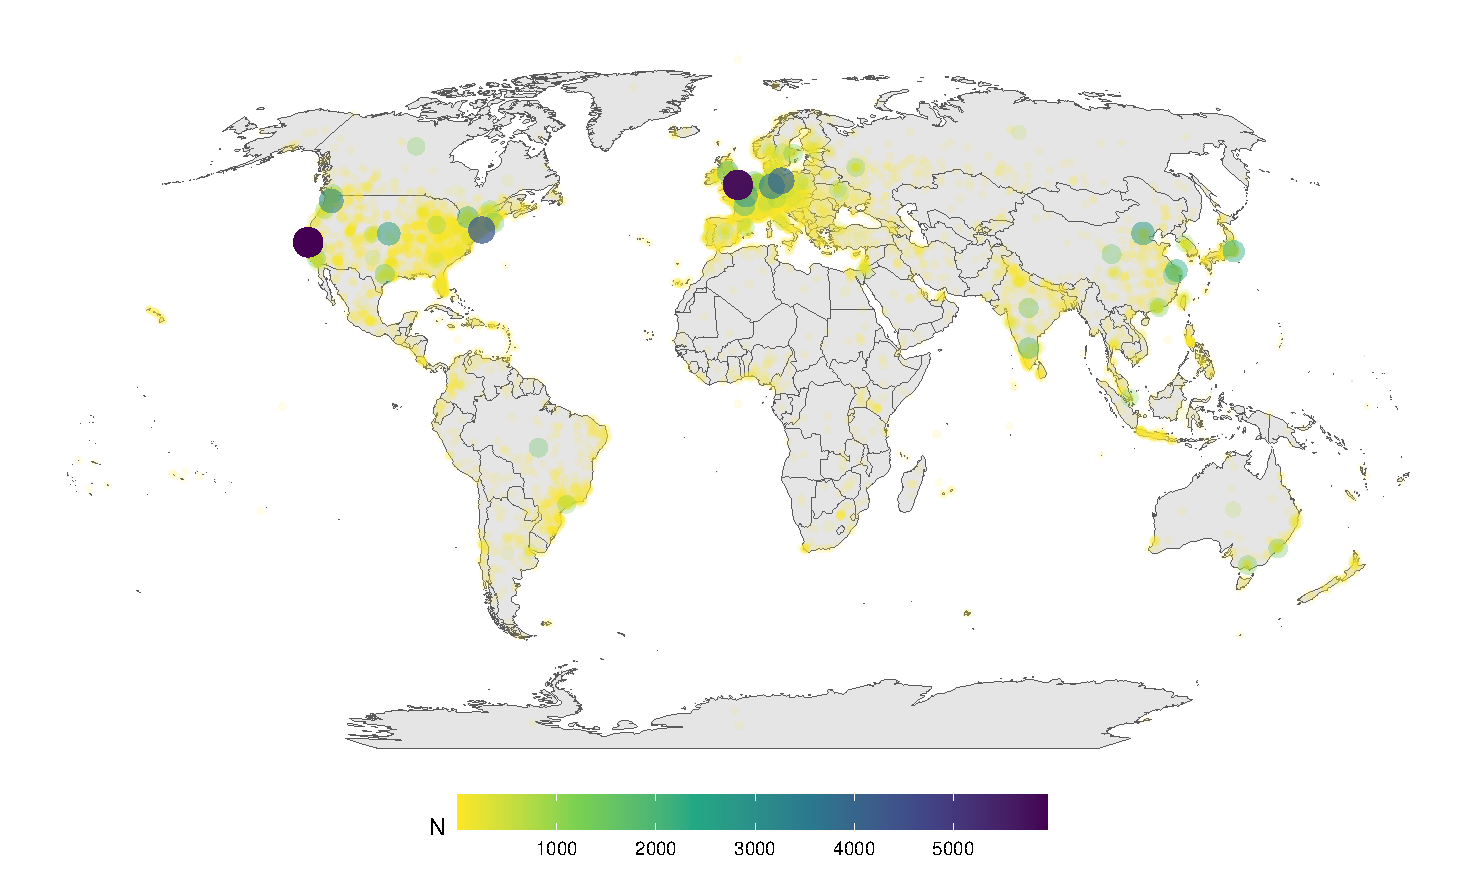
\includegraphics{goos/paper/figures/map_developers.pdf}
\end{frame}

\begin{frame}{Large variation in number of projects and developers}
\phantomsection\label{large-variation-in-number-of-projects-and-developers}
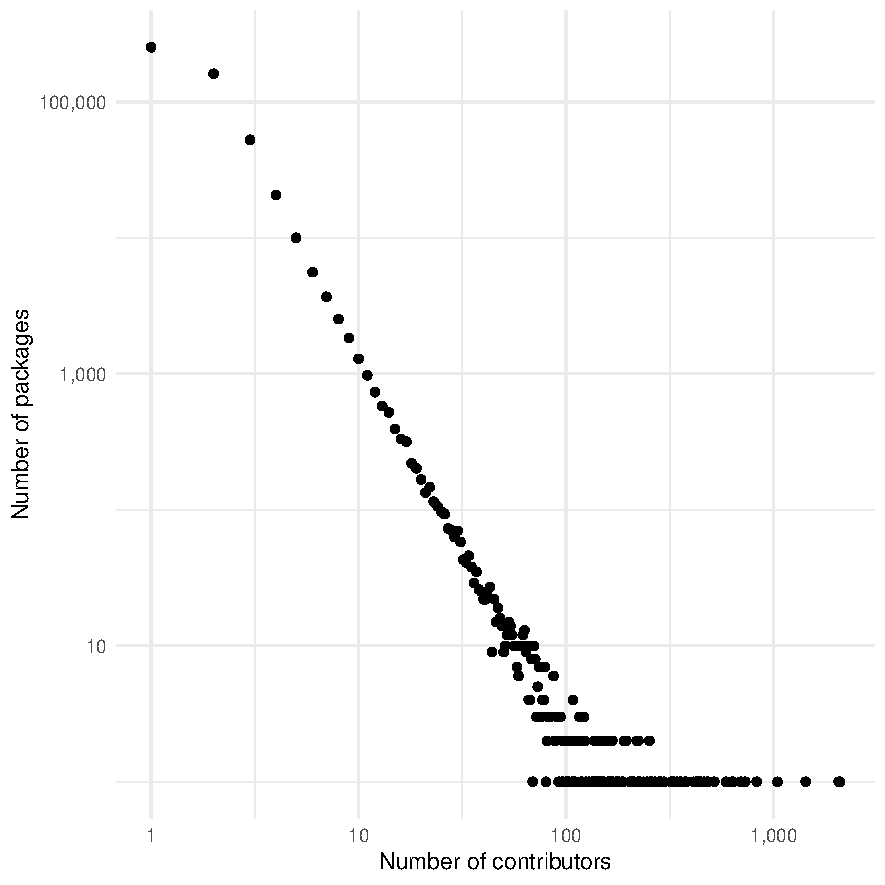
\includegraphics[width=0.5\textwidth,height=\textheight]{goos/paper/figures/contributors_per_package_ght.pdf}
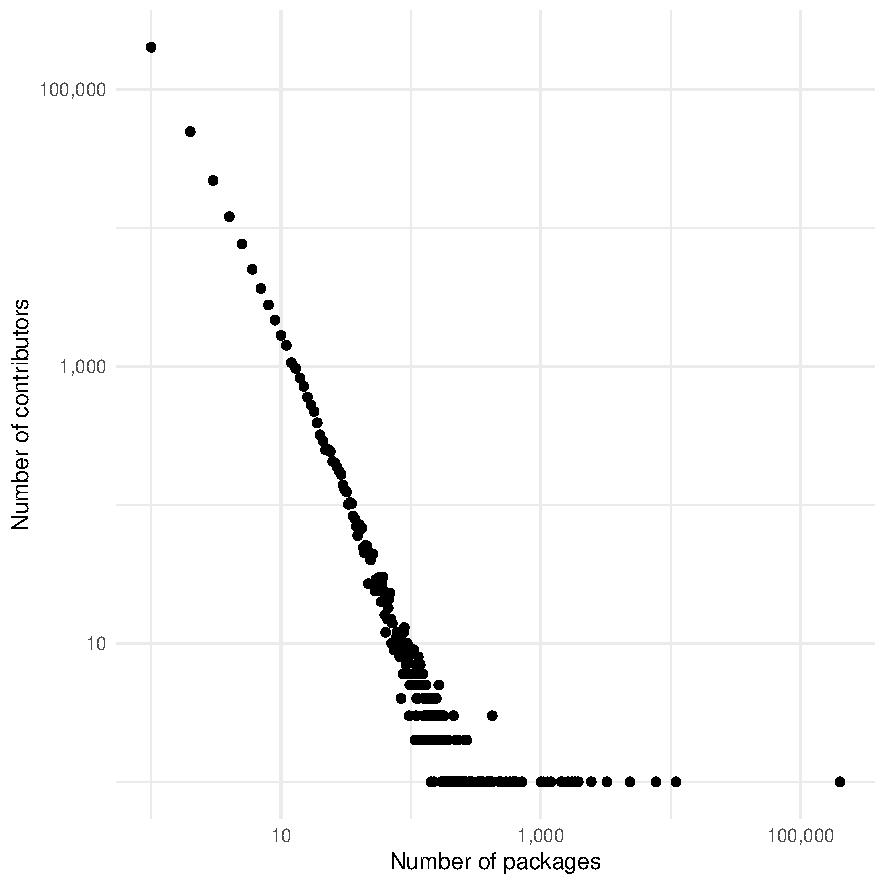
\includegraphics[width=0.5\textwidth,height=\textheight]{goos/paper/figures/packages_per_contributor_ght.pdf}
\end{frame}

\begin{frame}{With limits on how many projects one imports}
\phantomsection\label{with-limits-on-how-many-projects-one-imports}
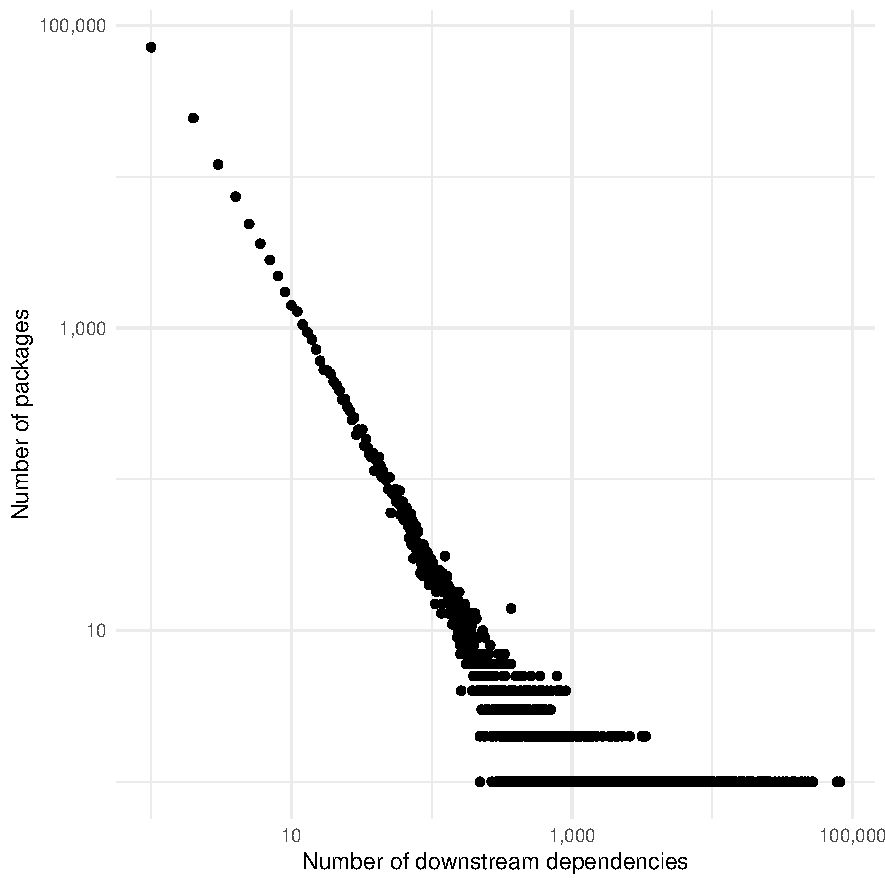
\includegraphics[width=0.5\textwidth,height=\textheight]{goos/paper/figures/dependencies_downstream.pdf}
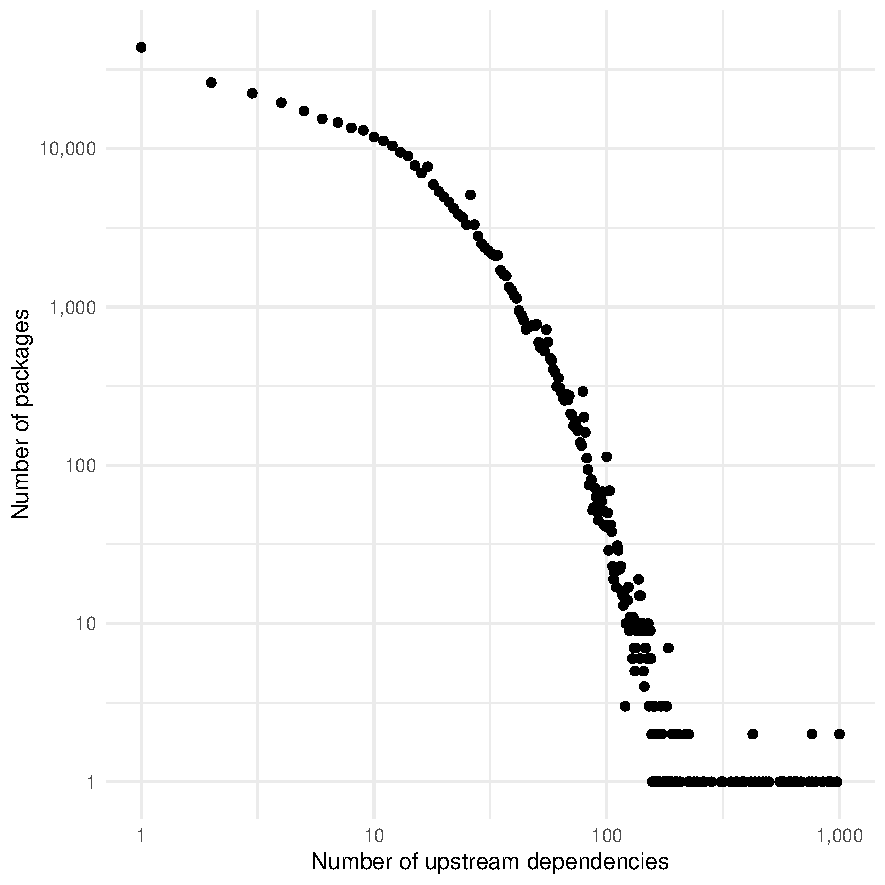
\includegraphics[width=0.5\textwidth,height=\textheight]{goos/paper/figures/dependencies_upstream.pdf}
\end{frame}

\begin{frame}{Measuring collalboration and dependencies}
\phantomsection\label{measuring-collalboration-and-dependencies}
\begin{figure}
    \begin{subfigure}{0.5\textwidth}
        \centering
        \begin{tikzpicture}[scale=0.9]
            % Nodes and arrows for the first figure
            \node[circle, draw] (A) at (0,2) {A};
            \node[circle, draw] (B) at (4,2) {B};
            \node[circle, draw] (C) at (4,0) {C};
            \node[rectangle, draw, minimum width=2cm, minimum height=1cm] (repo) at (0,0) {Repo}; % Adjust the width and height as needed

            \draw[->] (A) -- (repo);
            \draw[->] (B) -- (repo);
            \draw[->] (C) -- (repo);
        \end{tikzpicture}
        \caption{Developers committing to a repository.}
    \end{subfigure}%
    \begin{subfigure}{0.5\textwidth}
        \centering
        \begin{tikzpicture}
            % Nodes and lines for the first figure
            \node[draw, circle, minimum size=1cm] (A) at (0,1.5) {A};
            \node[draw, circle, minimum size=1cm] (B) at (0,0) {B};
            \node[draw, rectangle, minimum width=1.5cm, minimum height=1cm] (Repo1) at (0,-1.5) {Repo 1};

            \node[draw, circle, minimum size=1cm] (C) at (3,1.5) {C};
            \node[draw, circle, minimum size=1cm] (D) at (3,0) {D};
            \node[draw, rectangle, minimum width=1.5cm, minimum height=1cm] (Repo2) at (3,-1.5) {Repo 2};

            \draw[solid] (1.5,-1.5) -- (1.5,2.5);
            \draw[->] (Repo1.east) -- (Repo2.west);
        \end{tikzpicture}
        \caption{Dependency of repository 1 on repository 2 with the respective developers.}
    \end{subfigure}%
\end{figure}
\end{frame}

\begin{frame}{Gravity model of collaboration}
\phantomsection\label{gravity-model-of-collaboration}
Developer \(i\) and \(j\) collaborate with probability \[
\Pr(\text{Collaboration}_{ij}) = \exp(\alpha x_i + \beta x_j -\gamma\times\text{distance}_{ij})
\] Aggregate across city pairs \(d\) and \(o\): \[
E(N_{do}) = \exp(\alpha x_d + \beta x_o -\gamma\times\text{distance}_{do})
\] Estimate this with Poisson maximum likelihood.
\end{frame}

\begin{frame}{Three margins of collaboration}
\phantomsection\label{three-margins-of-collaboration}
\begin{enumerate}
\tightlist
\item
  Committing to the same project
\item
  Importing someone else's project
\item
  Members of the same organization
\end{enumerate}
\end{frame}

\begin{frame}{Strong localization of collaboration patterns}
\phantomsection\label{strong-localization-of-collaboration-patterns}
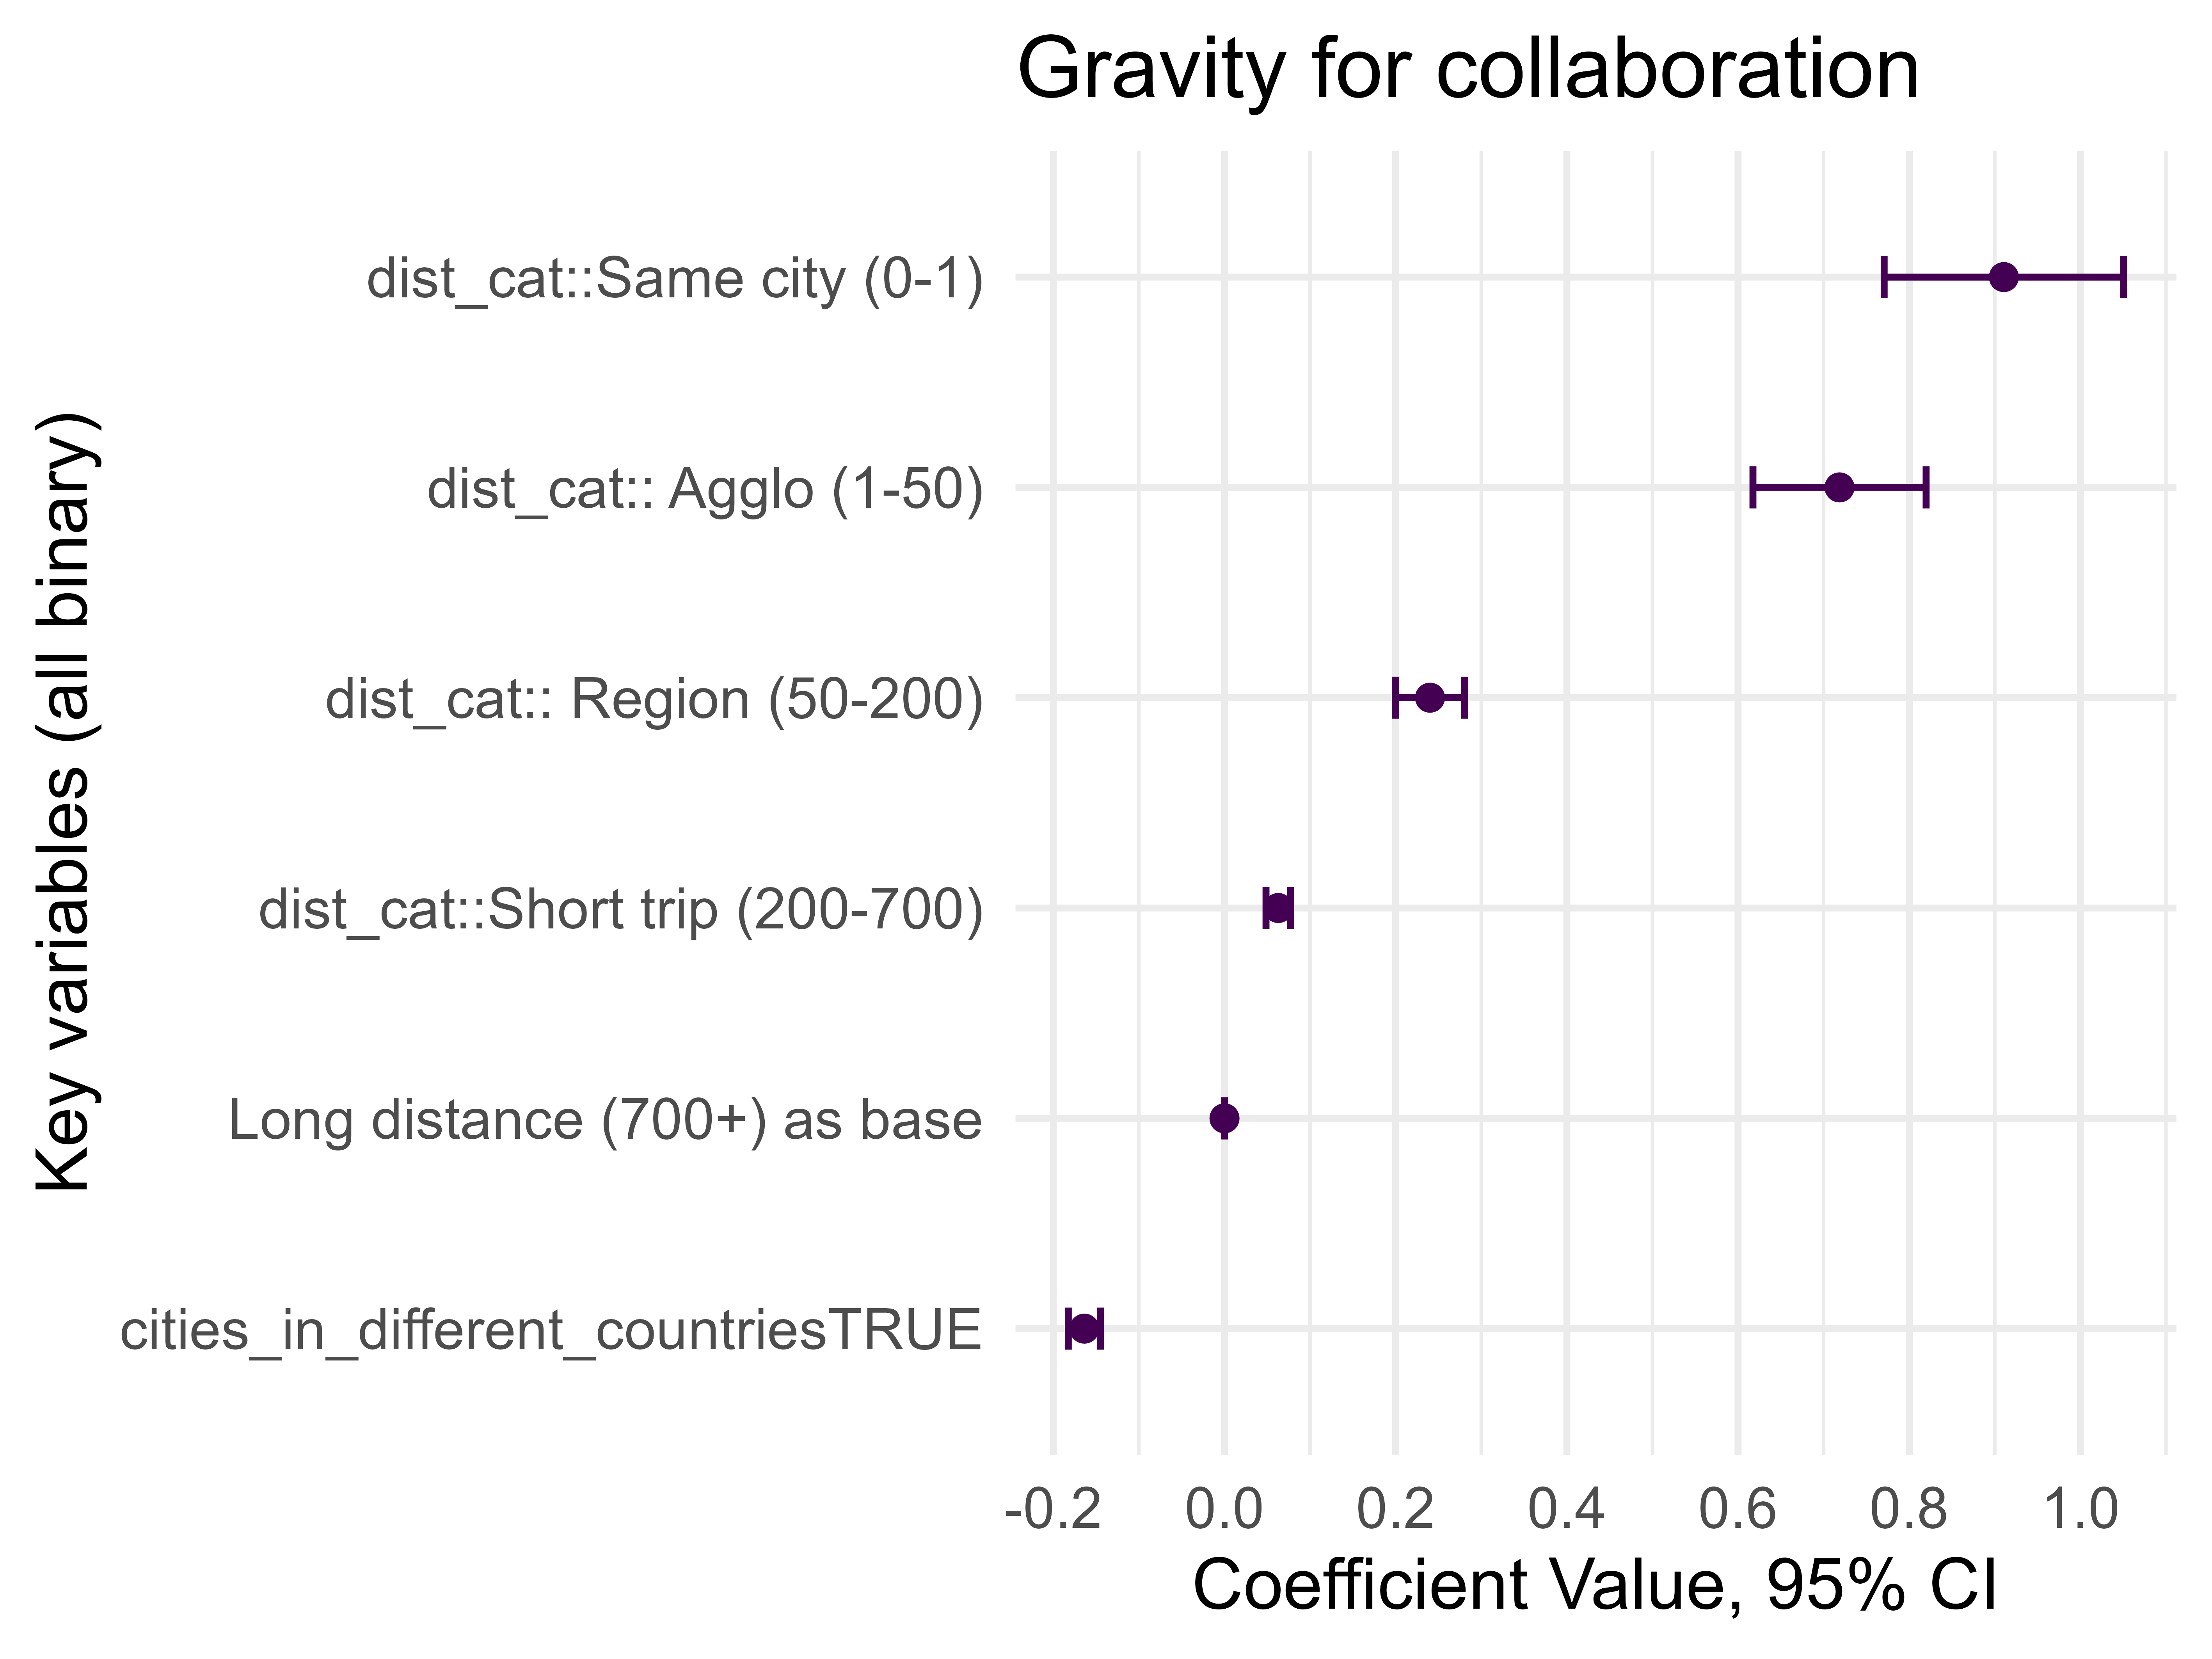
\includegraphics{goos/paper/figures/gravity_collaboration.png}
\end{frame}

\begin{frame}{No localization of dependencies}
\phantomsection\label{no-localization-of-dependencies}
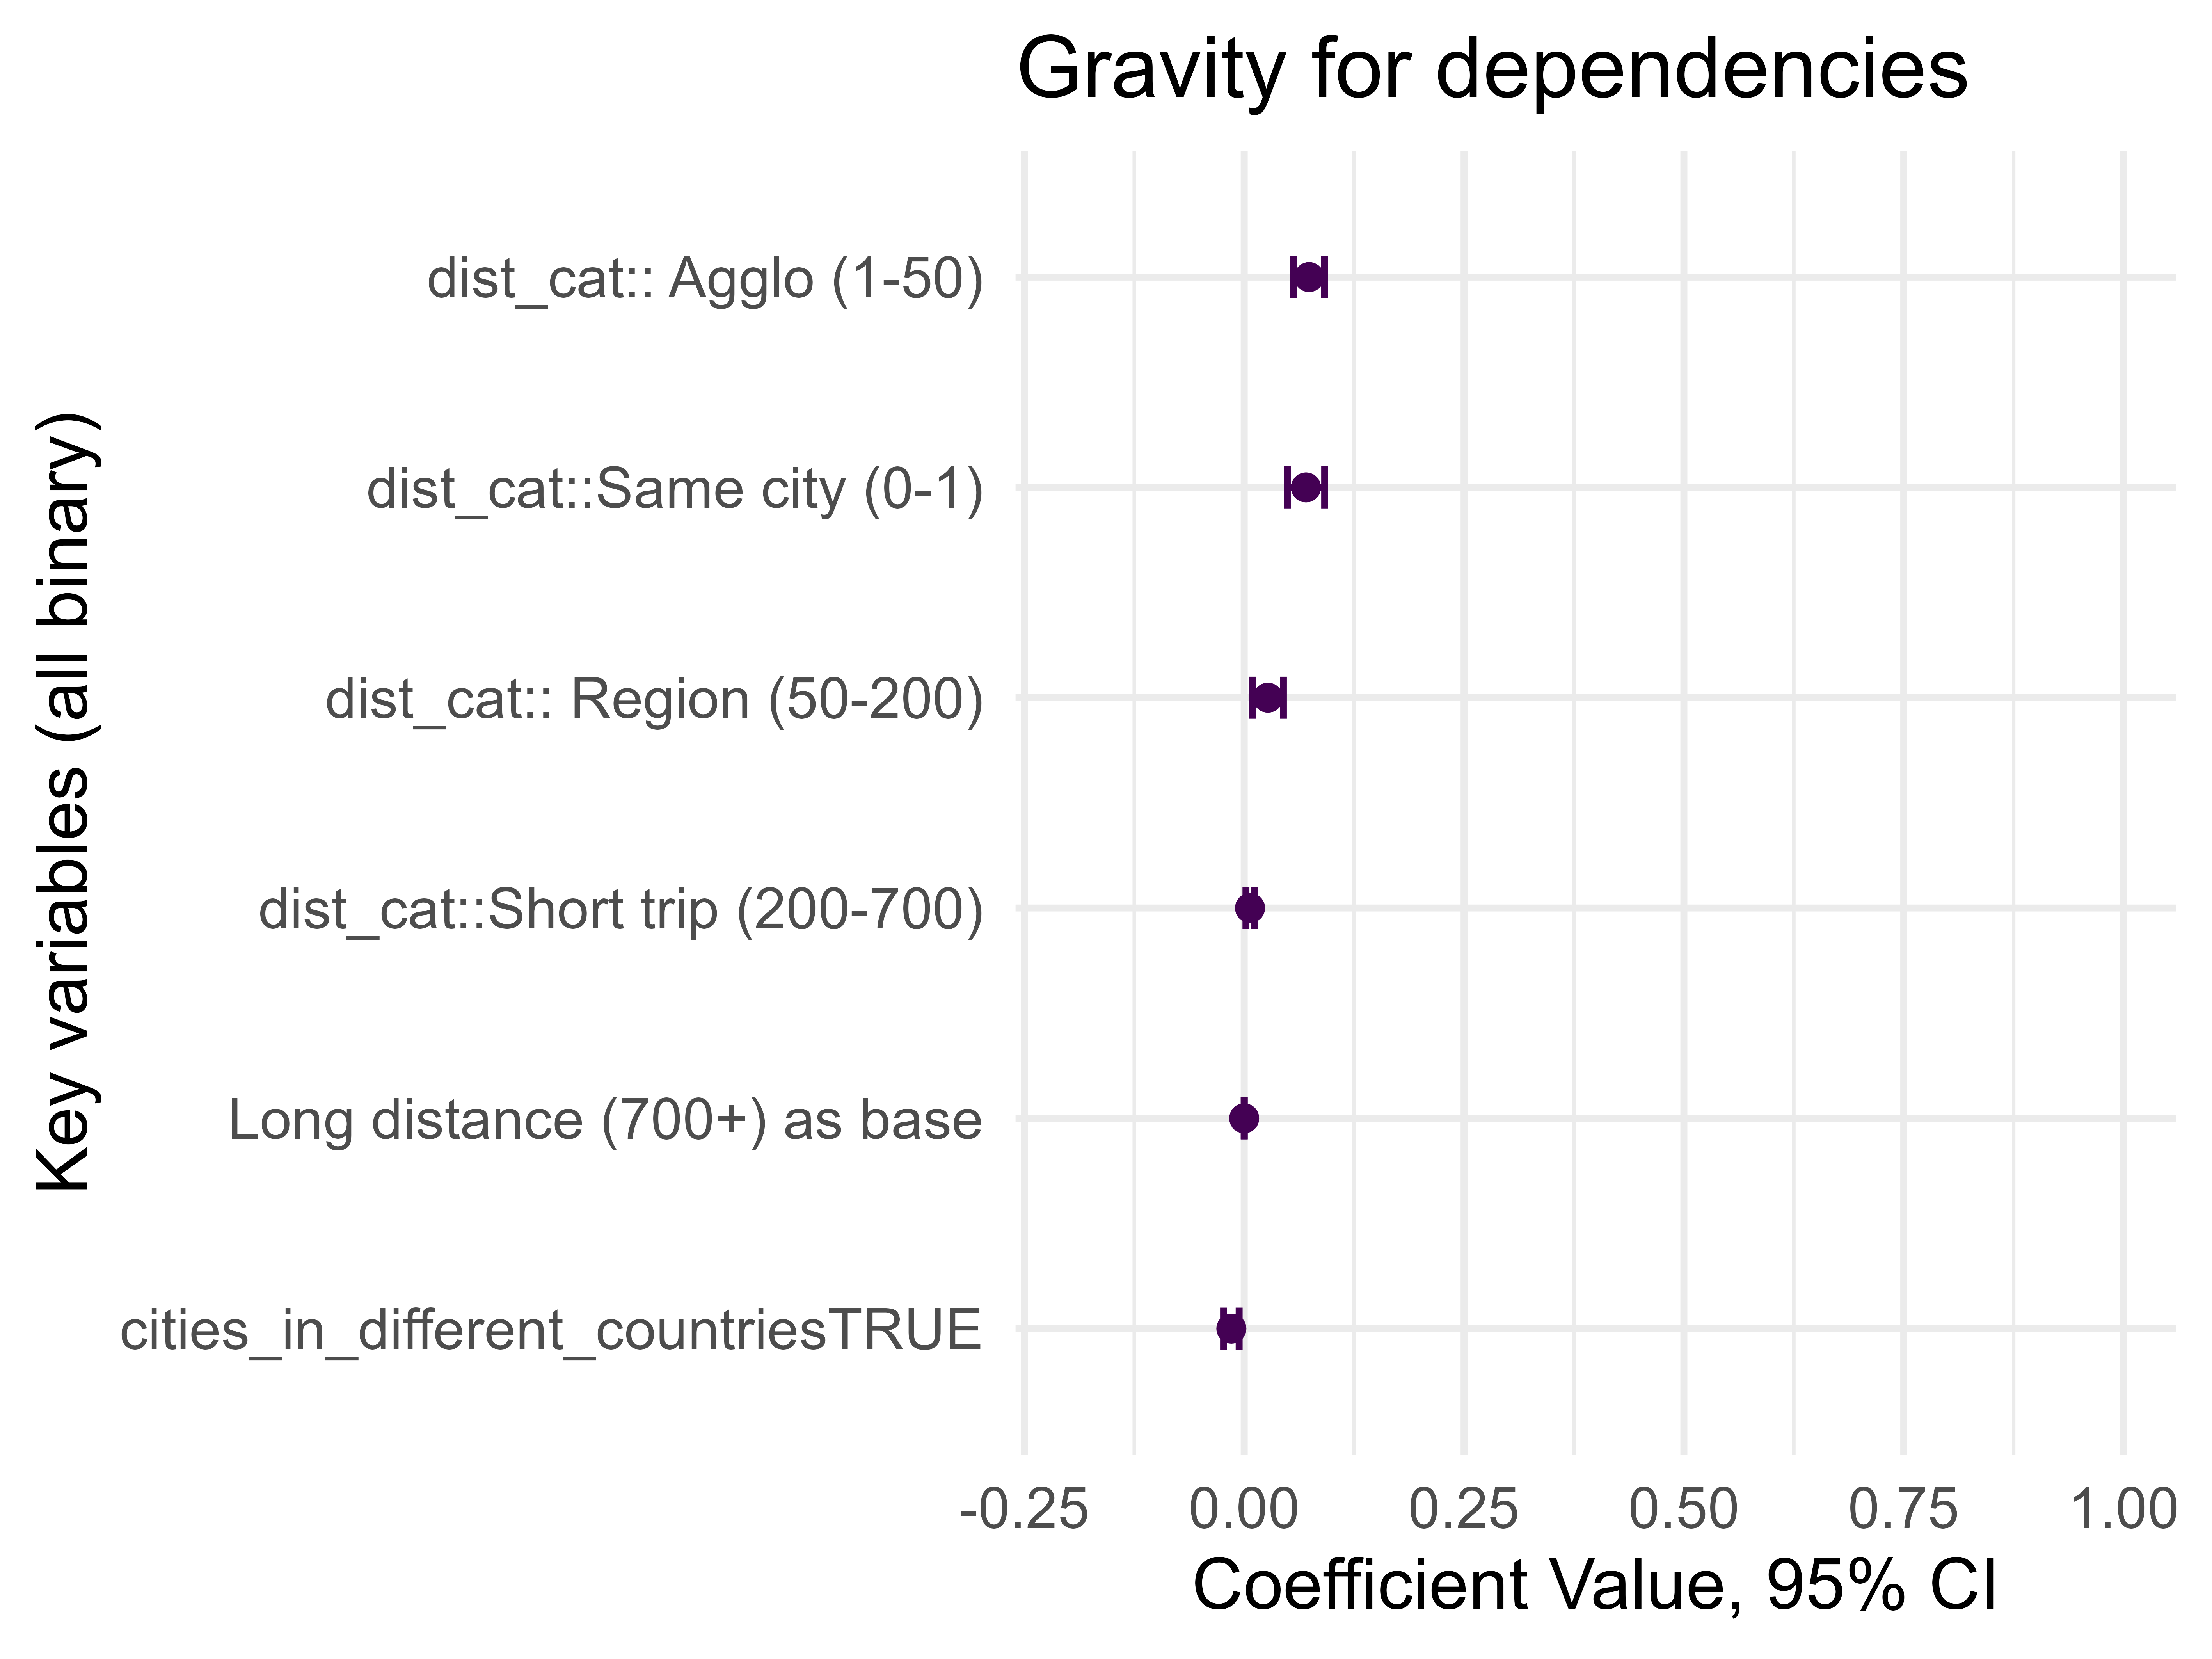
\includegraphics{goos/paper/figures/gravity_dependencies2.png}
\end{frame}

\begin{frame}{Diverse teams produce more popular software}
\phantomsection\label{diverse-teams-produce-more-popular-software}
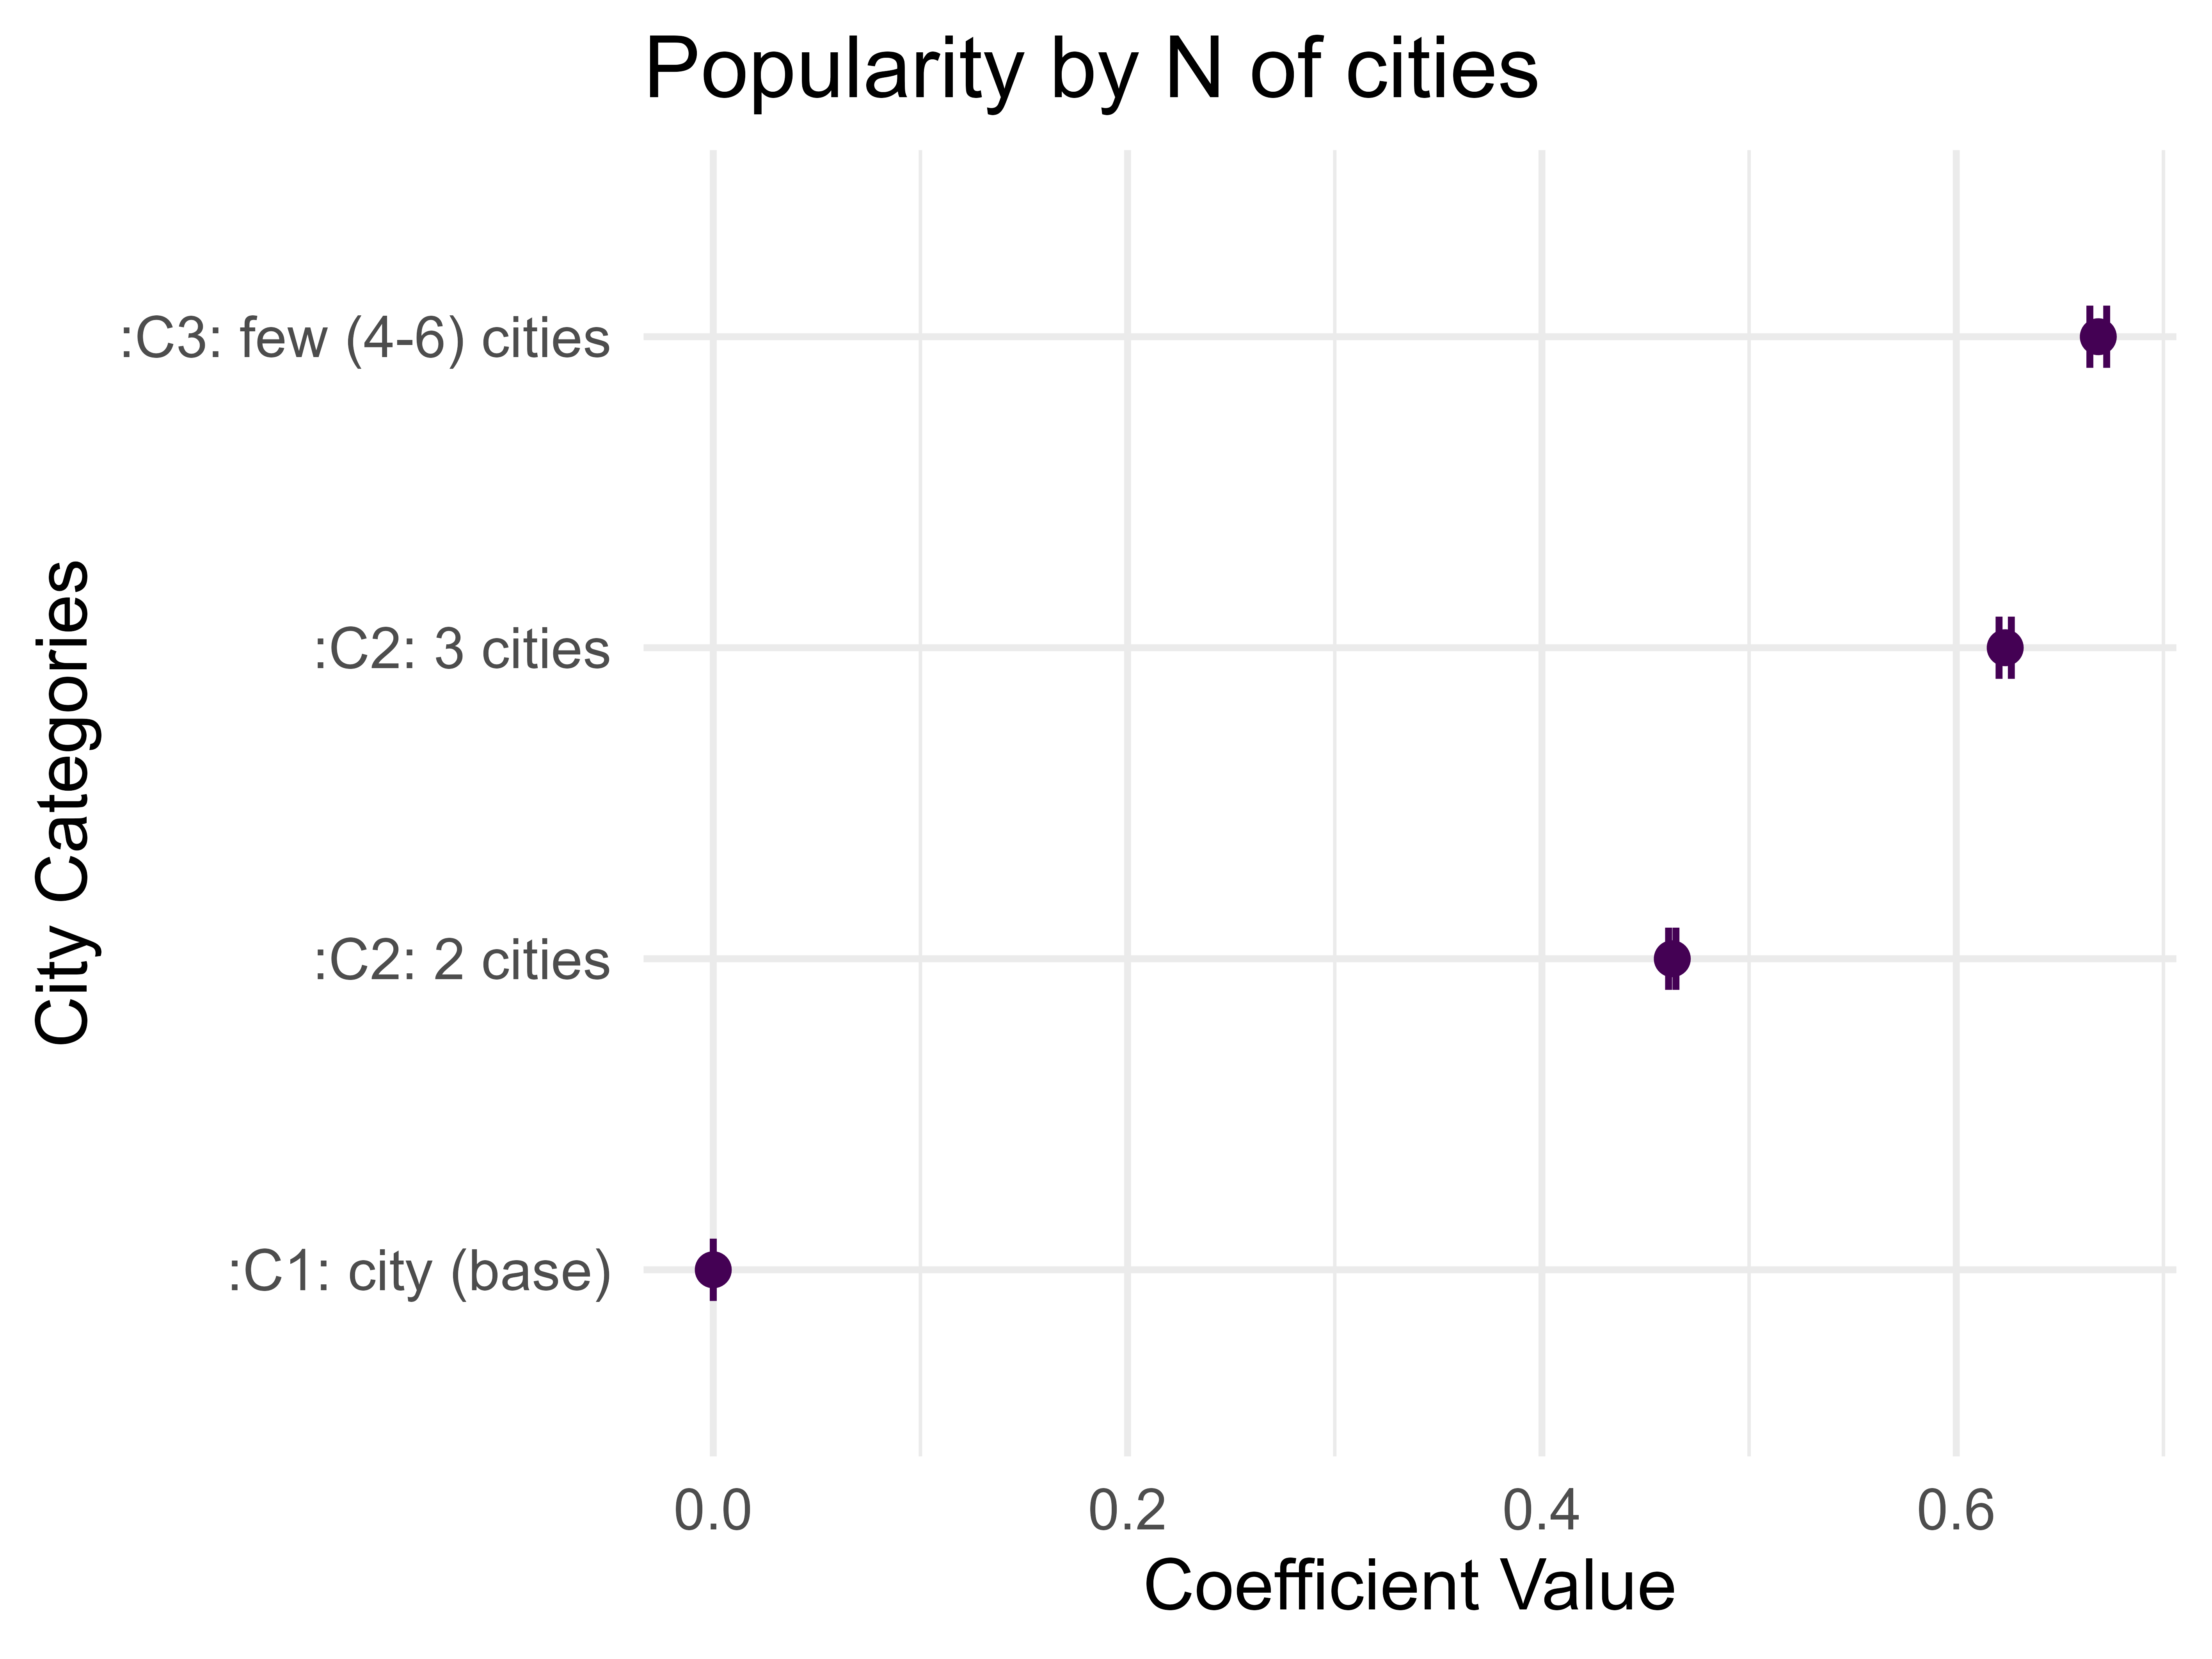
\includegraphics{goos/paper/figures/quality_dependencies_city_categories.png}
\end{frame}

\begin{frame}{Additional results}
\phantomsection\label{additional-results}
Organizations help overcome distance. Almost no distance penalty for
developers within the same GitHub organization.
\end{frame}

\section{\texorpdfstring{Bugs \emoji{lady-beetle}}{Bugs }}\label{bugs-1}

\begin{frame}{Model}
\phantomsection\label{model}
Long-standing question in economics: how does competition affect
innovation?

Model the special features of the OSS market.
\end{frame}

\begin{frame}{Special features}
\phantomsection\label{special-features}
\begin{enumerate}
\tightlist
\item
  Price is zero. Only compete in quality.
\item
  Software projects often start as a developer's own need.
\item
  Quality is only partly observable.
\item
  Collaboration is important.
\end{enumerate}
\end{frame}

\begin{frame}{Outline}
\phantomsection\label{outline}
\begin{enumerate}
\tightlist
\item
  Defining software quality
\item
  Producing quality
\item
  The market for software
\item
  Testable predictions
\item
  First evidence from GitHub
\end{enumerate}
\end{frame}

\section{Quality}\label{quality}

\begin{frame}{Software quality}
\phantomsection\label{software-quality}
Users have a use case \(X\).

Developers write code \(\bar z\) and tests \(\underline z\). Software
quality is random \(Z \sim U[\underline z, \bar z]\).

Software only works if \(Z > X\).

\[
\Pr(Z \text{works for} X) := \pi = \frac{\bar z - X}{\bar z - \underline z}.
\]
\end{frame}

\begin{frame}{Software quality}
\phantomsection\label{software-quality-1}
\begin{tikzpicture}[scale=4]
    % Draw axes
    \draw[->] (0,0) -- (1.2,0) node[right] {$Z$};
    \draw[->] (0,0) -- (0,1.2) node[above] {$X$};
    
    % Draw boundaries at 1
    \draw (1,0) -- (1,1);
    \draw (0,1) -- (1,1);
    
    % Draw interval [\underline{z}, \bar{z}]
    \fill[gray!50] (0.3,0) rectangle (0.7,1);
    \draw (0.3,0) -- (0.3,1);
    \draw (0.7,0) -- (0.7,1);
    
    % Label \underline{z} and \bar{z}
    \draw (0.3,0) node[below] {$\underline{z}$};
    \draw (0.7,0) node[below] {$\bar{z}$};
    
    % Draw 45-degree dotted line
    \draw[dotted] (0,0) -- (1,1);
    
    % Draw use case X = x_0
    \draw[red, thick] (0,0.5) -- (0.5,0.5); % Left of the 45-degree line
    \draw[red, ultra thick] (0.5,0.5) -- (1,0.5) node[right] {$X = x_0$}; % Right of the 45-degree line (thicker)
\end{tikzpicture}
\end{frame}

\begin{frame}{Probability of software working for a given use case}
\phantomsection\label{probability-of-software-working-for-a-given-use-case}
\begin{tikzpicture}[scale=1.5]  % Increase the scale value to increase the size of the figure
    % Axes
    \draw[thick, ->] (0,0) -- (5,0) node[below] {$x$};
    \draw[thick, ->] (0,0) -- (0,2) node[left] {$\pi(x)$};

    % x-axis labels
    \draw (1,0.1) -- (1,-0.1) node[below] {$\underline{z}$};
    \draw (3,0.1) -- (3,-0.1) node[below] {$\bar{z}$};

    % y-axis labels
    \draw (0.1,1) -- (-0.1,1) node[left] {1};

    % Line segments
    \draw[blue, thick] (0,1) -- (1,1); % Constant segment
    \draw[blue, thick] (1,1) -- (3,0); % Linear decreasing segment
    % Note: The line automatically stops at x=3

    % Dotted lines for clarity
    \draw[dotted] (1,1) -- (1,0);
    \draw[dotted] (3,1) -- (3,0);
\end{tikzpicture}
\end{frame}

\begin{frame}{The production of quality}
\phantomsection\label{the-production-of-quality}
Coding up to \(\bar z\) costs \(c(\bar z)\). Increasing and convex.

Testing up to \(\underline z\) costs \(t(\underline z)\). Increasing and
convex.

(Current results for \(t(z) = \tau c(z)\) with \(\tau \le 1\).)
\end{frame}

\begin{frame}{Cost of quality}
\phantomsection\label{cost-of-quality}
\begin{tikzpicture}
\begin{axis}[
    axis lines = left,
    xlabel = $z$,
    ylabel = {Cost},
    legend pos = north west,
    ymin=0,
    ymax=1,
    xmax=1,
    xmin=0,
    clip=false,
    domain=0:1
]
% Add c(z)
\addplot [
    domain=0:1, 
    samples=100, 
    color=red,
] {x^2};
\addlegendentry{$c(\bar{z})$}

% Add t(z)
\addplot [
    domain=0:1, 
    samples=100, 
    color=blue,
    style=dashed,
] {0.8*(x^2)};
\addlegendentry{$t(\underline{z})$}

% Add points for z_bar and z_underline
\draw[dotted] (axis cs:0.5,0) -- (axis cs:0.5,{0.5^2});
\node[label={90:{$\bar{z}$}},circle,fill,inner sep=2pt] at (axis cs:0.5,{0.5^2}) {};

\draw[dotted] (axis cs:0.3,0) -- (axis cs:0.3,{0.8*(0.3^2)});
\node[label={270:{$\underline{z}$}},circle,fill,inner sep=2pt] at (axis cs:0.3,{0.8*(0.3^2)}) {};

\end{axis}
\end{tikzpicture}
\end{frame}

\section{Market}\label{market}

\begin{frame}{Three market environments}
\phantomsection\label{three-market-environments}
\begin{enumerate}
\tightlist
\item
  Do-it-yourself: developer writes code for own use. \(X=u\) is known.
\item
  Shared platform: developer writes code for others. \(X\sim F\) is
  unknown.
\item
  Competition: \(n\) developers write code for the same set of users.
\end{enumerate}
\end{frame}

\begin{frame}{The DIY economy}
\phantomsection\label{the-diy-economy}
The developer maximizes \[
\max_{\underline z, \bar z} \frac{\bar z- u}{\bar z - \underline z} - t(\underline z) - c(\bar z)
\] subject to \(\underline z, \bar z \ge 0\) and
\(\underline z \le \bar z\).
\end{frame}

\begin{frame}{The platform economy}
\phantomsection\label{the-platform-economy}
Assume developer can capture \(\phi \ll 1\) share of the value of the
software.

She maximizes \[
\max_{\underline z, \bar z} \phi \int \frac{\bar z- x}{\bar z - \underline z} dF(x) - t(\underline z) - c(\bar z)
\] subject to \(\underline z, \bar z \ge 0\) and
\(\underline z \le \bar z\).
\end{frame}

\begin{frame}{Competition}
\phantomsection\label{competition}
Two-sided market with \(U\) users and \(D\) developers.

Each user meets \(n\) developers at random.

They choose the software with the highest \(\underline z\).
\end{frame}

\begin{frame}{Competition}
\phantomsection\label{competition-1}
With \(G(z)\) is the distribution of tested software quality in the
marketplace, \[
\Pr(z_j \text{ wins}|x_i,\underline z_j,n) = G^{n-1}(\underline z_j),
\]
\end{frame}

\begin{frame}{Developer's problem}
\phantomsection\label{developers-problem}
Maximize \[
\max_{\underline z, \bar z} \frac {\phi nU}{D} \int \frac{\bar z- x}{\bar z - \underline z} dF(x) G^{n-1}(\underline z)
 - t(\underline z) - c(\bar z) 
\]
\end{frame}

\begin{frame}{Collaboration}
\phantomsection\label{collaboration}
Collaboration helps overcome diminishing returns to coding. With \(n\)
collaborators, the total coding cost up to \(\bar z\) is \[
C(\bar z) :=
\min_{\{z_i\}} \sum_{i=1}^n
    c_i(z_i)
    \,\text{ s.t. }\,
    \sum_{i=1}^n z_i \ge \bar z
\] \[
n c(\bar z/n) < c(\bar z)
\]

There may be increasing returns to collaboration: lower marginal cost
\(\to\) higher demand \(\to\) more individual contribution.
\end{frame}

\section{Predictions}\label{predictions}

\begin{frame}{Predictions on testing}
\phantomsection\label{predictions-on-testing}
\begin{enumerate}
\tightlist
\item
  DIY projects are not fully tested.
\item
  Shared projects are.
\end{enumerate}
\end{frame}

\begin{frame}{Predictions on code quality}
\phantomsection\label{predictions-on-code-quality}
\begin{enumerate}
\tightlist
\item
  Standalone projects are limited by developer's own need. Diminishing
  returns to quality.
\item
  Shared projects have higher quality. Constant returns to quality.
\item
  Competition increases quality. Increasing returns to quality.
\end{enumerate}
\end{frame}

\begin{frame}{Predictions on collaboration}
\phantomsection\label{predictions-on-collaboration}
\begin{enumerate}
\tightlist
\item
  Collaborative project may have \emph{more} individual contribution.
\item
  Especially in shared projects.
\end{enumerate}
\end{frame}

\begin{frame}{Measurement}
\phantomsection\label{measurement}
Six biggest languages on GitHub: JavaScript, Python, Java, Ruby, PHP,
and C++.

Contribution: number of commits per developer per project.

Compare the \emph{same} developer in the \emph{same} language across
projects.

Developer skill: average number of stars per solo-authored project.
\end{frame}

\begin{frame}{Larger projects are written by more people}
\phantomsection\label{larger-projects-are-written-by-more-people}
\begin{figure}
\centering
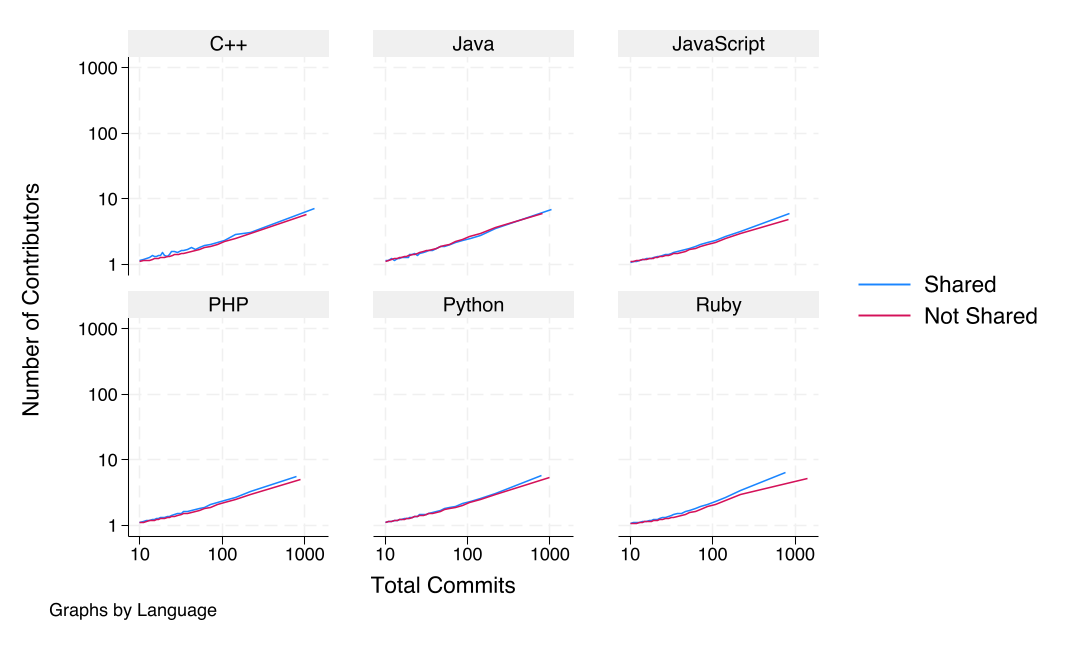
\includegraphics{figures/n_contributors_by_commits.png}
\caption{Larger projects by more people}
\end{figure}
\end{frame}

\begin{frame}{Larger projects are more popular}
\phantomsection\label{larger-projects-are-more-popular}
\begin{figure}
\centering
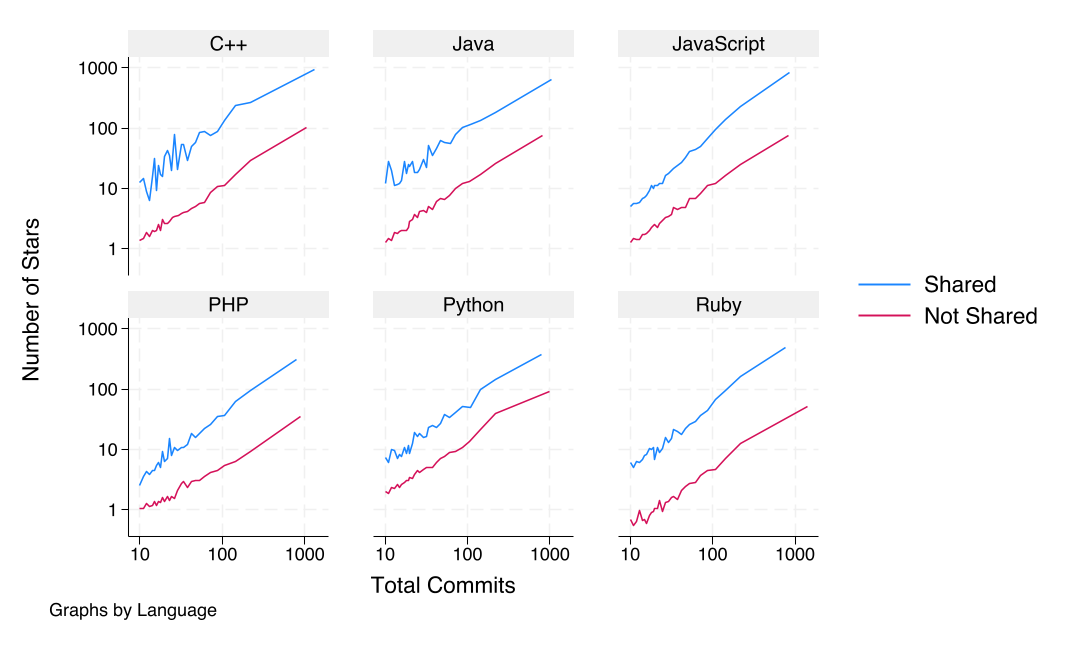
\includegraphics{figures/n_stars_by_commits.png}
\caption{Larger projects are more popular}
\end{figure}
\end{frame}

\begin{frame}{Larger projects have more bug discovery}
\phantomsection\label{larger-projects-have-more-bug-discovery}
\begin{figure}
\centering
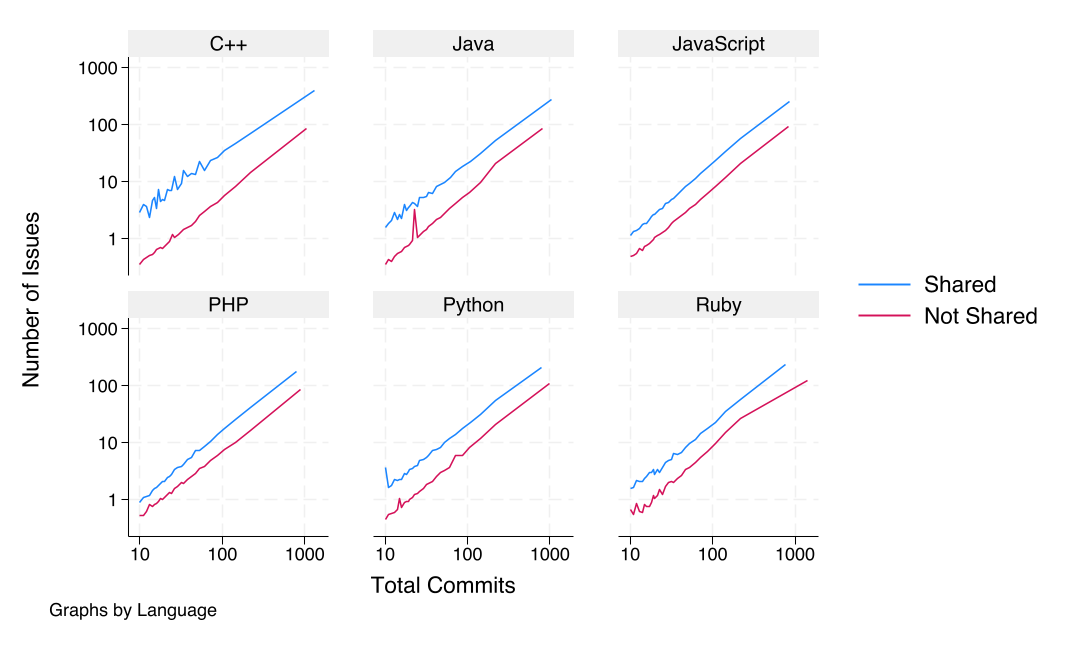
\includegraphics{figures/n_issues_by_commits.png}
\caption{Larger projects have more bug discovery}
\end{figure}
\end{frame}

\begin{frame}{Larger projects solve a larger share of issues}
\phantomsection\label{larger-projects-solve-a-larger-share-of-issues}
\begin{figure}
\centering
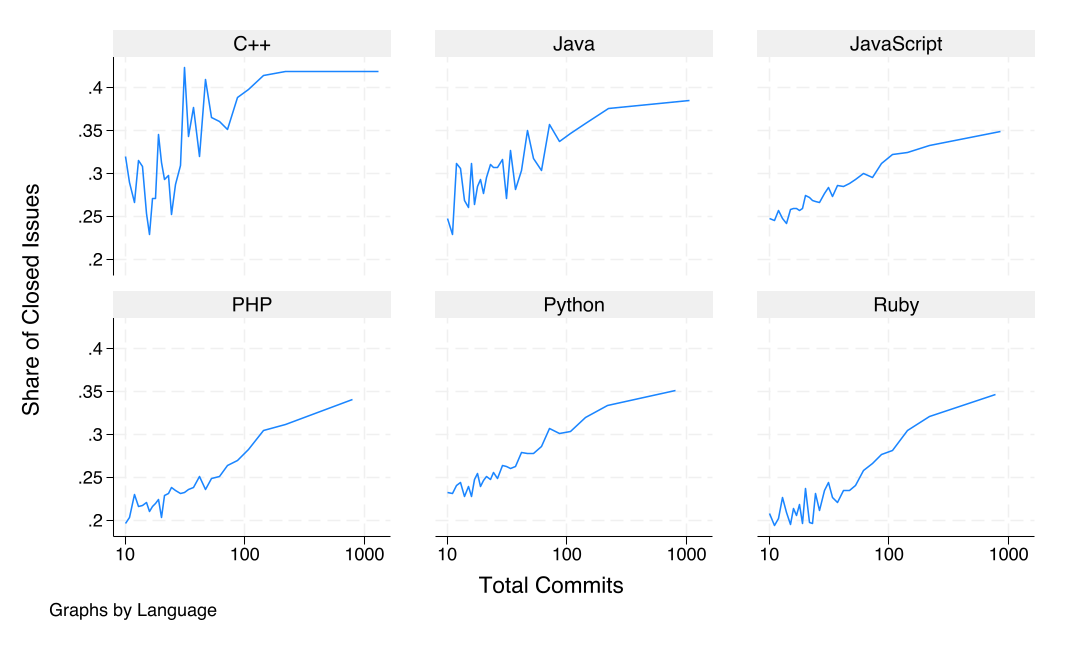
\includegraphics{figures/share_closed_by_commits.png}
\caption{Larger projects solve a larger share of issues}
\end{figure}
\end{frame}

\begin{frame}{Better developers contribute more to shared projects}
\phantomsection\label{better-developers-contribute-more-to-shared-projects}
\begin{figure}
\centering
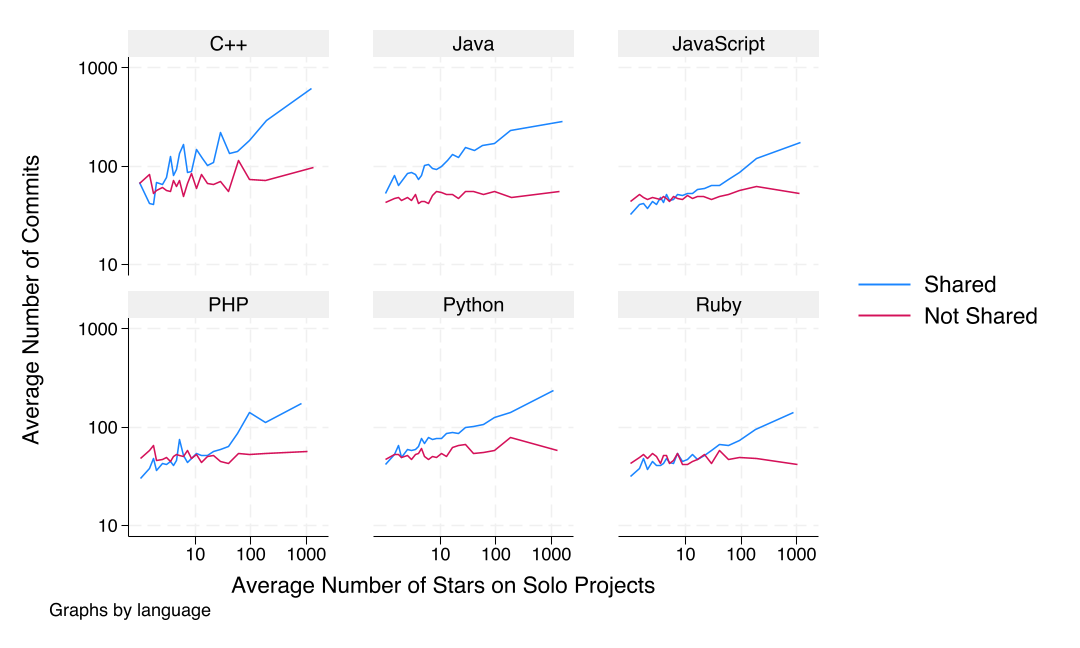
\includegraphics{figures/avg_n_commits_by_quality.png}
\caption{Better developers contribute more to shared projects}
\end{figure}
\end{frame}

\begin{frame}{Shared projects are better quality}
\phantomsection\label{shared-projects-are-better-quality}
\begin{figure}
\centering
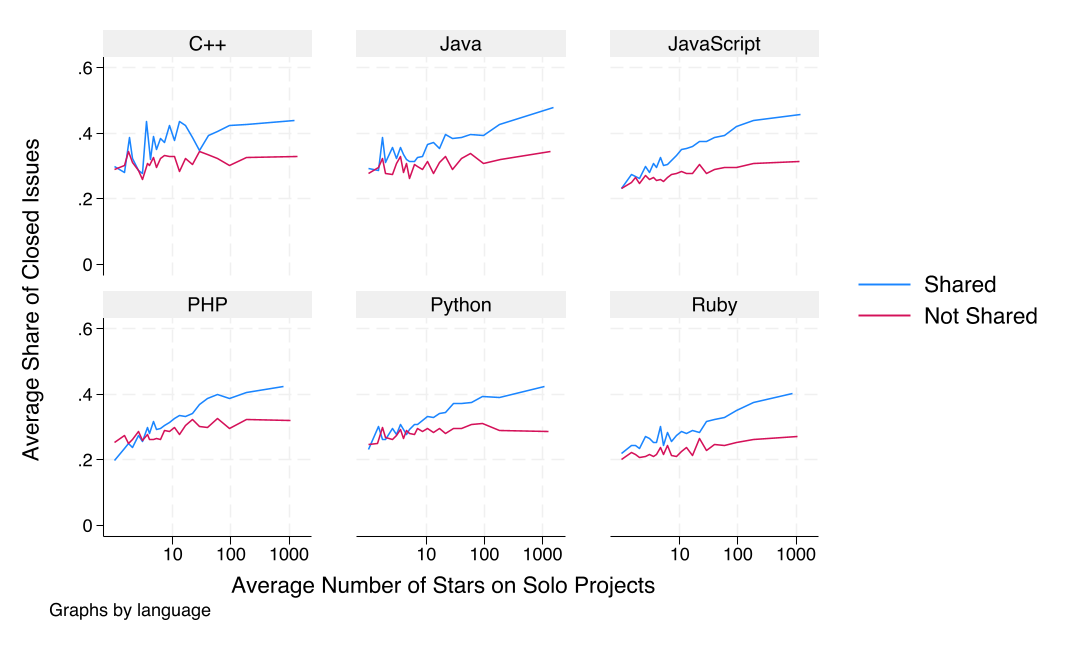
\includegraphics{figures/avg_share_closed_by_quality.png}
\caption{Shared projects are better quality}
\end{figure}
\end{frame}

\begin{frame}{Good developers contribute more to shared projects}
\phantomsection\label{good-developers-contribute-more-to-shared-projects}
\begin{tabular}{lcccc} \hline
 & (1) & (2) & (3) & (4) \\
VARIABLES & Private projects & DIY projects & Shared projects & Popular projects \\ \hline
 &  &  &  &  \\
Developer skill & 0.0101*** & 0.00840*** & 0.0867*** & 0.110*** \\
 & (0.00108) & (0.00126) & (0.00195) & (0.00362) \\
No. contributors (log) &  & 0.0450*** & 0.0265*** & -0.0680*** \\
 &  & (0.00388) & (0.00478) & (0.00638) \\
Constant & 3.233*** & 3.197*** & 3.125*** & 3.243*** \\
 & (0.00281) & (0.00326) & (0.00442) & (0.0134) \\
 &  &  &  &  \\
Observations & 361,196 & 629,039 & 514,259 & 136,503 \\
 R-squared & 0.002 & 0.002 & 0.038 & 0.037 \\ \hline
\multicolumn{5}{c}{ Robust standard errors in parentheses} \\
\multicolumn{5}{c}{ *** p$<$0.01, ** p$<$0.05, * p$<$0.1} \\
\end{tabular}

\end{frame}

\begin{frame}{Popular projects attract better developers}
\phantomsection\label{popular-projects-attract-better-developers}
\begin{tabular}{lccc} \hline
 & (1) & (2) & (3) \\
VARIABLES & Commits & Commits & Commits \\ \hline
 &  &  &  \\
Shared on a platform (dummy) & 0.0731*** & 0.0457*** & 0.0281*** \\
 & (0.00789) & (0.0108) & (0.0107) \\
Has downstream projects &  & 0.0370*** & 0.0314*** \\
 &  & (0.0100) & (0.00998) \\
Has 5 or more stars (dummy) &  &  & 0.116*** \\
 &  &  & (0.00775) \\
Constant & 3.055*** & 3.054*** & 2.889*** \\
 & (0.0112) & (0.0113) & (0.0163) \\
 &  &  &  \\
Observations & 172,495 & 172,495 & 172,495 \\
 R-squared & 0.680 & 0.680 & 0.681 \\ \hline
\multicolumn{4}{c}{ Robust standard errors in parentheses} \\
\multicolumn{4}{c}{ *** p$<$0.01, ** p$<$0.05, * p$<$0.1} \\
\end{tabular}

\end{frame}

\begin{frame}{Next steps}
\phantomsection\label{next-steps}
Measure test coverage.

Interaction with users: bug reports, feature requests.

Sorting into collaboration.
\end{frame}

\begin{frame}{Get in touch}
\phantomsection\label{get-in-touch}
@korenmiklos

@gaborbekes

@julianhinz
\end{frame}

\end{document}
